\chapter{Proof Systems}
\label{sec:proof-theory}
\section{Zero Knowledge Proofs}
\subsection*{Overview}
This concept was introduced by Goldwasser et al.~\cite{goldwasser1985knowledge} in 1985, which provided a widely used definition of zero-knowledge protocols: "A zero-knowledge proof allows one party (the prover) to convince another party (the verifier) of the truth of a statement without disclosing any information other than the fact that the statement is indeed true".\\To ensure this the prover constructs a new statement, known as a proof of knowledge, whose truth implies the truth of the original statement, without divulging any private information.

First we will explain Interactive proofs systems, required for explaining SNARKs, and their role in zero-knowledge proofs.

\subsection{Interactive Proof System}
An interactive proof system models an interaction between two parties: the prover and the verifier. The prover wants to convince the verifier of the truth of a statement, and the verifier aims to verify the statement without being deceived.

Interactive zero-knowledge proof systems are a subset of interactive proofs systems. All zero-knowledge proofs must satisfy the following three properties, where $\mathcal{L}$ is a language and $x$ a public statement, and a true public statement is $x\in\mathcal{L}$~\cite{fortnow1989complexity}:
\begin{itemize}
    \item \textbf{Completeness}. If the statement is true, and the prover possesses a valid proof, then the the verifier will be convinced of its truth. Thus, $\forall x\in\mathcal{L}$, the verifier will accept the proof.
    \item \textbf{Soundness}. If the statement is false, a dishonest prover $P$ cannot convince an honest verifier except with a small probability. In other words, $\forall x\notin\mathcal{L}$, the honest verifier $V$ cannot be convinced otherwise with probability $>1/2^{|x|}$.
    \item \textbf{Zero-Knowledge}. The verifier learns only the truth or falsehood of the statement and gains no additional information. Thus, the statement is enough to convince the verifier that the prover knows the necessary knowledge.
\end{itemize}

The protocol involves a public parameter $x$ belonging to the language $\mathcal{L}$, known to both the prover $P$ and the verifier $V$, and a private parameter, the witness, $w$.
The protocol proceeds through several steps:
\begin{enumerate}
    \item The prover $P$ sends a commitment of the private input (witness) to $V$.
    \item The verifier $V$ creates a random challenge and sends it to $P$.
    \item The prover $P$ sends to the verifier $V$ the evaluated proofs of the challenge to $V$.
    \item The verifier verifies these evaluations.
\end{enumerate}

These interactions are conducted a sufficient number of times, decided by the verifier.

The verifier finally accepts the proof if the prover responded correctly to enough challenges, which is possible if the prover knows the private input.

We can see that there is a continuos interaction between the prover and the verifier. Next, non-interactive proof systems will be introduced in which the number of interactions between the prover and the verifier will be only one.

\subsection{SNARKs}
Now, we can define SNARKs, \textit{succinct non-interactive argument of knowledge}~\cite{10.1145/3335741.3335757}. SNARKs can be used in large computations for providing integrity of the results~\cite{nitulescu2020zk}.

The correctness of some proofs need to be publicly verified, preferably by multiple parties. A way to overcome this problem is to make proofs non-interactive, thus, public verifiable. In this solution, the challenges are created by the prover. So, continuous interaction between the prover and verifier is no longer necessary.

The proof system of the SNARK is:

\begin{itemize}
    \item \textbf{succinct}. The size of the proof is small compared to the statement being proved, so we can generate a small proof of a large computation.
    \item \textbf{non-interactive}. There is no interaction between the prover and the verifier.
    \item \textbf{argument.} This property means that the proof convinces the verifier of the truth of the statement, assuming that the prover is computationally bounded (i.e., limited to polynomial-time computations). This allows us to relax some constraints compared to proofs of knowledge, as an exponentially powerful prover could potentially cheat. The key difference between an argument of knowledge and a proof of knowledge is that the former assumes the prover's computational limitations.
    \item \textbf{knowledge-sound.} The proof provided by the prover must be constructed using a witness associated with the statement being proved. So the proof not only demonstrate integrity of the statement but also knowledge of some secret information. 
    In the context of NP statements\footnote{A NP statement is a statement about a problem for which we don't know has an easy solution, but if we have a solution, we can easily verify its correctness.}, a polynomial-time prover cannot solve the problem unless it already knows a witness. Knowledge-soundness guarantees that if the prover can generate a valid proof, it must possess knowledge of a valid witness.
\end{itemize}

A zk-SNARK, \textit{zero-knowledge succinct non-interactive arguments of knowledge}, can be used to generate proofs without revealing nothing more (witnesses) than the proof. A zk-SNARK is defined as follows:
\begin{enumerate}
    \item Setup. A trusted third party (TTP) or a secure multi-party computation (MPC)~\cite{goldreich1998secure} generates a public common reference string $S$ that will be used in the proof generation and verification.
    \item Proof generation. Given $S$, the statement $x$ and the witnesses $w$, the prover generates the proof $\pi$.
    \item Proof verification. The verifier takes a verification key $vk$ from $S$, the statement $x$ and the proof $\pi$, determines if accept or reject the proof.
\end{enumerate}

\subsection{Arithmetic circuits}
Most zkSNARK proof systems operate over arithmetic circuits. This means that the computations must be "converted" into arithmetic circuits. These circuits are described using directed acyclic graphs whose vertices and edges represent gates and wires.

There is some similarity to boolean circuits. In boolean circuits, the operations are logical operations like AND, and OR, while on arithmetic circuits, the operations are addition and multiplication. Unlike boolean gates who operates on bits, arithmetic circuit operates on elements of the finite field $\mathbb{F}_p$.

Each gate of the circuit can be an input gate, an output gate, a constant gate, an addition gate or a multiplication gate. An example of an arithmetic circuit is provided in Figure~\ref{fig:arithmetic-circuit}. Let's consider an arithmetic circuit $\mathcal{G}: \mathbb{F}_p^3\longrightarrow\mathbb{F}_p$, that computes the polynomial $f(x_1,x_2,x_3):=x_3\cdot(x_1+x_2)$.

\begin{figure}[h]
    \centering
    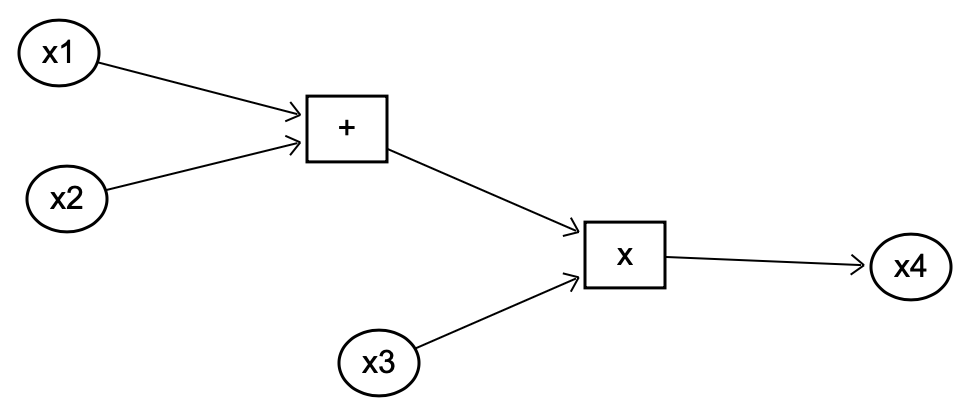
\includegraphics[width=0.7\textwidth]{graphics/arithmetic-circuit.png}
    \caption{Arithmetic circuit for computing $x_4:=x_3\cdot(x_1+x_2)$}
    \label{fig:arithmetic-circuit}
\end{figure}

In this example, $x_1$, $x_2$ and $x_3$ are input gates, $x_4$ is an output gate and there is a multiplication and an addition gate.


\section{PLONK}
\label{sec:plonk}
\subsection*{Overview}
PLONK, \textit{Permutations over Lagrange-bases for Oecumenical Noninteractive arguments of Knowledge}, was introduced by Gabizon et al. in 2019~\cite{gabizon2019plonk}. It is a zkSNARK proving system and the one that will be used and explained in this thesis.

\subsection{Constraint system}
In~\cite{gabizon2019plonk}, a constraint system $\mathcal{C}$ over $\mathbb{F}_p$ is introduced, allowing the representation of arithmetic circuits. These circuits can contain gates with at most two inputs each, and output gates that can be connected to any number of other gates.\\
Let $m$ represent the number of wires and $n$ the number of gates, excluding private input/output gates. Let $\textbf{x}\in\mathbb{F}_p^m$ be the wire assignment\footnote{A \textbf{wire assignment} referes to the assignment of specific values from the field $\mathbb{F}_p$ to the wires in an arithmetic circuit.}. Let $\textbf{a},\textbf{b},\textbf{c}\in[m]^n$ be the left, right and output vector sequence of each gate in the circuit $\mathcal{G}$, respectively. Additionally, let $\textbf{q}_\textbf{L},\textbf{q}_\textbf{R},\textbf{q}_\textbf{O},\textbf{q}_\textbf{M},\textbf{q}_\textbf{C}\in\mathbb{F}_p^n$, where each \textbf{q} term represents a selector vector\footnote{A \textbf{selector vector} is a constant used to control the behavior of the arithmetic circuit based on the type of gate being evaluated.} in $\mathbb{F}_p$ used to define constraints based on the gate type.\\
Thus, the PLONK constraint at every gate $i\in[n]$ must satisfy
\begin{equation}
    \left(\textbf{q}_\textbf{L}\right)_i\cdot\textbf{x}_{\textbf{a}_i}+ \left(\textbf{q}_\textbf{R}\right)_i\cdot\textbf{x}_{\textbf{b}_i} + \left(\textbf{q}_\textbf{O}\right)_i\cdot\textbf{x}_{\textbf{c}_i} + \left(\textbf{q}_\textbf{M}\right)_i\cdot\left(\textbf{x}_{\textbf{a}_i}\textbf{x}_{\textbf{b}_i}\right) + \left(\textbf{q}_\textbf{C}\right)_i=0
    \label{eq:plonk-constraint}
\end{equation}

For example, from the vector sequence \textbf{a}, we set $\textbf{a}_i:=j$, where $j\in[m]$ is the index of the value $\textbf{x}_j$ assigned to the left input of the $i$ gate, in other words, for each gate $i$ in the circuit, we are selecting a specific wire to be its left input.

To build a \textbf{multiplation gate} we set $\left(\textbf{q}_\textbf{L}\right)_i=0$, $\left(\textbf{q}_\textbf{R}\right)_i=0$, $\left(\textbf{q}_\textbf{M}\right)_i=1$, $\left(\textbf{q}_\textbf{O}\right)_i=-1$, $\left(\textbf{q}_\textbf{C}\right)_i=0$, and we get the following constraint for a gate $i$
\[\textbf{x}_{\textbf{a}_i}\textbf{x}_{\textbf{b}_i}-\textbf{x}_{\textbf{c}_i}=0.\]\\
Similary, for an \textbf{addition gate}, we set $\left(\textbf{q}_\textbf{L}\right)_i=1$, $\left(\textbf{q}_\textbf{R}\right)_i=1$, $\left(\textbf{q}_\textbf{M}\right)_i=0$, $\left(\textbf{q}_\textbf{O}\right)_i=-1$, $\left(\textbf{q}_\textbf{C}\right)_i=0$, resulting in the constraint:
\[\textbf{x}_{\textbf{a}_i}+\textbf{x}_{\textbf{b}_i}-\textbf{x}_{\textbf{c}_i}=0.\]\\
Lastly, for a \textbf{constant gate}, we set $\left(\textbf{q}_\textbf{L}\right)_i=1$, $\left(\textbf{q}_\textbf{R}\right)_i=0$, $\left(\textbf{q}_\textbf{M}\right)_i=0$, $\left(\textbf{q}_\textbf{O}\right)_i=0$, $\left(\textbf{q}_\textbf{C}\right)_i=-c_i$, and the corresponding constraint is
\[\textbf{x}_{\textbf{a}_i}-c_i=0.\]\\
To summarize the initial proces of PLONK: 
\begin{enumerate}
    \item We build the arithmetic circuit based on the PLONK constraint of the program, where each operation of the circuit (addition, multiplication) corresponds to a gate in the circuit.
    \item The arithmetic circuit is translated into a constraint system, formed by all the contraints used to build the circuit.
\end{enumerate}

\subsubsection*{Copy constraints}
Up until now, we have been focused on how to build gates within the arithmetic circuit. However, we are not connecting them, we are missing the wiring. Copy constraints ensure that the outputs of some gates correctly map to the inputs of subsequent gates.

\subsubsection*{Example}
Let's illustrate the PLONK protocol with an example. Consider the arithmetic circuit from Figure~\ref{fig:arithmetic-circuit-plonk}, which computes $v_4:=v_1\cdot v_2+v_3$. In this circuit, $v_1, v_2, v_3$ are private inputs (the witnesses), while $v_4$ is the public input.
\begin{figure}[htbp]
    \centering
    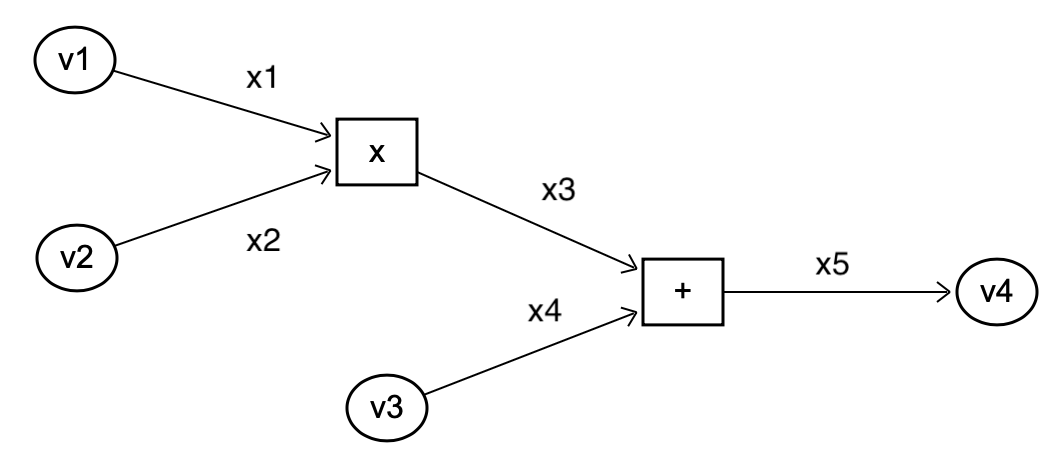
\includegraphics[width=0.7\textwidth]{graphics/arithmetic-circuit-plonk.png}
    \caption{Arithmetic circuit for computing $v_4:=v_1\cdot v_2+v_3$}
    \label{fig:arithmetic-circuit-plonk}
\end{figure}
In this arithmetic circuit we have 3 private input gates $(v_1, v_2, v_3)$, $m=5$ wires and $n=3$ gates, let $i=1$ be the multiplication gate, $i=2$ the addition gate, and $i=3$ the output gate, the sequence vectors \textbf{a}, \textbf{b}, \textbf{c }$\in[5]^3$ are\[\textbf{a}:=(1,3,5),\textbf{ b}:=(2,4,5),\textbf{ c}:=(3,5,5).\]\\
To make it more clear, let's demonstrate the process for gate $i=2$ (addition gate). The left wire $x_3=\textbf{x}_{\textbf{a}_2}$, where $\textbf{a}_2$ denotes the index of the left input wire. Similary, the right input wire $x_4=\textbf{x}_{\textbf{b}_2}$, and the output wire $x_5=\textbf{x}_{\textbf{c}_2}$, and so on for each component of the vector sequence.\\
By assigning the corresponding values to the selector vectors, depending on the type of gate as explained earlier, we get the following constraints:
\begin{align*}
    x_1\cdot x_2-x_3=0 \\
    x_3+x_4-x_5=0 \\
    x_5-v4=0
\end{align*}

Next, we need to establish the connections between different gates. In this case, it consists in connecting the multiplication gate with the addition gate and the addition with the output gate. Thus, we define the copy constraints for these cases:
\begin{align*}
    a_2=c_1 \\
    c_2=a_3
\end{align*}

\subsection{Compressing Constraints}
There is a property about polynomials, called the \textit{Schwartz-Zippel lemma}~\cite{zippel1979probabilistic, barbara2021reinforced} widely used in zero-knowledge proving systems, including Plonk. This lemma affirms that if two polynomials $P$ and $Q$ result in the same value when evaluated at some random point $a$, then it's highly probable that the two polynomials are identical.

To use this property we convert the constraint system into a polynomial expression that is true if the constraint system is satisfied.

\subsubsection*{Lagrange interpolation}
Plonk uses Lagrange interpolation to convert the constraint system to a polynomial. We define polynomials $a(i),b(i),c(i)$ to interpolate the values in \textbf{x} with the vectors \textbf{a}, \textbf{b}, \textbf{c}, and $Q_L(i),Q_R(i),Q_O(i),Q_M(i),Q_C(i)$ to interpolate $\textbf{q}_\textbf{L},\textbf{q}_\textbf{R},\textbf{q}_\textbf{O}, \textbf{q}_\textbf{M}, \textbf{q}_\textbf{C}$ for each $i$.\\
Now, using Equation~\eqref{eq:plonk-constraint} we express the constraint as a polynomial:
\begin{equation}
    Q_\text{L}(i)a(i)+Q_\text{R}(i)b(i)+Q_\text{O}(i)c(i)+Q_\text{M}a(i)b(i)+Q_\text{C}(i)=0
\end{equation}

\subsection{Polynomial commitments}
A polynomial commitment can be used to verify evaluations of a polynomial without needing access to entire polynomial itself. In other words, let's define a commitment $c$ representing the polynomial $P(x)$. There is a proof that can convince you of the value of $P(z)$ for some point $z$, without revealing the polynomial $P(x)$ itself.

The mathematical details of the polynomial commitment scheme is out of the scope of this thesis, requiring the exclusion of certain details. For a more detailed explanation look at~\cite{10.1007/978-3-642-17373-8_11}.

Intuitively, there are some equations between the polynomials that need to be checked. In Plonk, the prover need to commit to multiple polynomials. Although, the prover and the verifier could handle all the commitments one by one, in~\cite{gabizon2019plonk}, these polynomials are commited within a single step.
These commitments are evaluated at some random point $z$, along with proofs indicating that these evaluations are correct. Finally, the equations are applied to these evaluations rather than the original polynomials.\\
Thus, the final proof is just some commitments and the evaluations, and can be checked with a few equations.